\documentclass[11pt,a4paper,parskip=half ]{scrartcl}
\usepackage[utf8]{inputenc}
\usepackage[ngerman]{babel}
\usepackage{amsmath}
\usepackage{amsfonts}
\usepackage{amssymb}
\usepackage{graphicx}
\usepackage{xcolor}
\usepackage{float}
\usepackage{graphicx}
\usepackage{hyperref}

\author{Aaron Winziers - 1176638}
\title{Einführung in die Computergrafik SS 2019\\\LARGE{Übungsblatt 3}}

\begin{document}
	\maketitle
	
	\section*{Aufgabe 1}
$
R = 
\begin{bmatrix}
    \cos(\frac{\pi}{6}) & -\sin(\frac{\pi}{6}) & 0	\\
    \sin(\frac{\pi}{6}) & \cos(\frac{\pi}{6}) & 0	\\
    0 & 0 & 1	\\
\end{bmatrix}= 
\begin{bmatrix}
\frac{\sqrt{3}}{2}) & -0,5 & 0	\\
0,5 & \frac{\sqrt{3}}{2} & 0	\\
0 & 0 & 1	\\
\end{bmatrix}
\newline
S = 
\begin{bmatrix}
0,5 & 0 & 0	\\
0 & 0,5 & 0	\\
0 & 0 & 1	\\
\end{bmatrix}
\newline
T_{1} = 
\begin{bmatrix}
1 & 0 & -2	\\
0 & 1 & -1.5	\\
0 & 0 & 1	\\
\end{bmatrix}
\newline
T_{2} = 
\begin{bmatrix}
1 & 0 & 2	\\
0 & 1 & 1,5	\\
0 & 0 & 1	\\
\end{bmatrix}
\newline
T_{1}\times R\times S\times T_{2} =
\begin{bmatrix}
0.433 & -0.250 & -1.509 \\
0.250 & 0.433 & -0.350 \\
0.000 & 0.000 & 1.000
\end{bmatrix}
$\\
\vspace{.5cm}\\
Formel für Rotation($R$) von Folie 17, Skalierung($S$) von Folie 16, und Translation($T_1, T_2$) von Folie 15. Die Translationen sind notwendig um dafür zu sorgen dass das die Ecke unten Links des Rechtecks an Position (1.5, 2) bleibt. Das Recheck erst an den Punkt (0,0) gebracht werden, sonst würde (1.5, 2) auch um (0,0) rotiert werden.
\newpage
Aaron Winziers - 1176638

\section*{Aufgabe 2}
	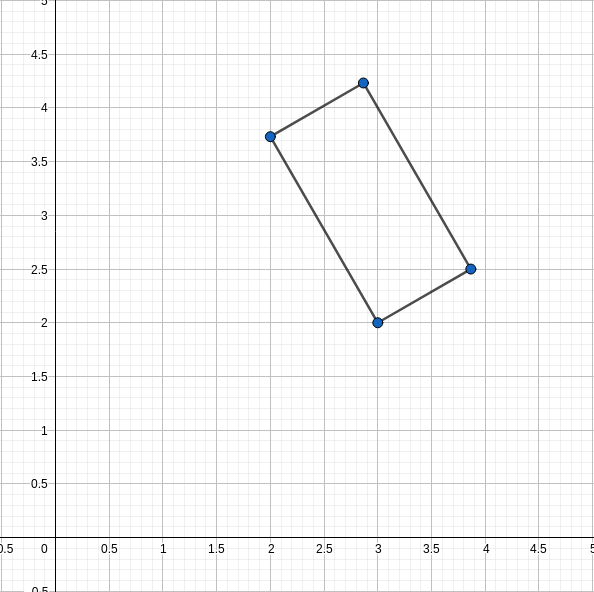
\includegraphics[width=.75\textwidth]{Aufgabe2.png}
	\\
	Punkte wurden in Python berechnet. Um Skript auszuführen runme.sh ausführen.
\end{document}